\documentclass[runningheads, 12pt]{report}
\usepackage{graphicx}
\graphicspath{{images/}}
\usepackage{subfig}
\usepackage{subfloat}
\usepackage{amsmath}
\usepackage{listings}
\usepackage{color}

\begin{document}	
	\title{Project: Building an Integer ALU - Report 2}
	\author{John Yamamoto 
		\and Alan Zacatula
		\and  Samuel Wait}
	\date{Due October 31, 2023}

	\maketitle
	
	\section{Introduction}
	
	For the second step of the project, already installed the virtual environment with Verilog and GTK Wave, so we did not need to worry about that. Instead, we were able to jump right into coding, compiling, and testing the new 4-bit Binary ALU functions (And, Nand, Or, Nor, Xor, Xnot, Not, and Shifter) and 4-bit Arithmetic  ALU operations (Addition, Subtraction, and Multiplication with carry-in and carry-out circuits)and test benches required for the assignment in Verilog. We then generated the simulation circuit waveforms using GTK Wave within the established Ubuntu virtual environment according to project specifications.   
	
	\section{And Circuit}
	
	The 4-bit And circuit works essentially the same as a 1-bit And circuit, but instead takes a 4-bit input and output rather than a 1-bit input and output. The circuit takes the 4-bit input, x and y, and performs an & operation on them, assigning result to the 4-bit output, o and ending the module. The test bench was a bit more complicated but is similar to the test benches for the circuits from the previous report. We first code a clock that pulses every 5 nanoseconds by changing the clock value to a 0 or 1 each with each pulse, and loading in new 4-bit x and y inputs every 10 nanoseconds, so every 2 pulses of the clock. For every new 4-bit x and y input, the And circuit is run and returns a 4-bit output o. We then have code to dump all the outputs into a .vcd file that GTK Wave uses to generate the waveforms and a string output to the screen that shows the clocks time, 4-bit x and y inputs, and the 4-bit o output, after which the module is ended. The And circuit Verilog source code and test bench is shown below:

\begin{lstlisting}[language=Verilog, caption={And Circuit Verilog}]
module and_gate_4bit(x, y, o);	//module name

input [3:0] x, y;		//inputs
output [3:0] o;			//outputs

assign o = x & y;		//o = x and y

endmodule			//end
\end{lstlisting}

\begin{lstlisting}[language=Verilog, caption={And Circuit Test Bench}]
//module name
module and_gate_4bit_tb;	

  /* Make a regular pulsing clock. */	
  //tracks every 5 ns
  reg clk = 0;
  //every 5 ns clk either 1 or 0S
  always #5 clk = !clk;			
  
  //inputs
  reg [3:0] x = 0;	
  reg [3:0] y = 0;
  //load new values
  initial begin				
  //every 10 nanoseconds
    	 x = 4'b1111;			
    # 10 x = 0; 
    	 y = 4'b1111;
    # 10 x = 4'b1111;			
    # 10 y = 4'b0110;
    # 10 $finish;
  end
  //output
  wire [3:0] o;			
  //call for gate module	
  and_gate_4bit a0(x, y, o);
  
  //code for gtkwave
  initial begin				
    $dumpfile("and_gate_4bit.vcd");
    $dumpvars(0,clk);
    $dumpvars(1,x);
    $dumpvars(2,y);
    $dumpvars(3,o);
  end
  
  initial				
  //prints to screen when values change
    $monitor("At time %t, x(%b), y(%b) = o(%b)",  
    		$time, x, y, o);
endmodule //test
\end{lstlisting}

	\section{Nand Circuit}
	
	The 4-bit Nand circuit uses the same code structure as the And circuit, but instead uses the Not operator to negate the & operation on 4-bit inputs x and y. The module then assigns the result of the Nand code to the 4-bit output o and ends the module. The test bench for this circuit works the same as the And circuit test bench, as we first code a clock that pulses every 5 nanoseconds that alternates the clock value between 0 and 1, changing the 4-bit x and y values every time the clock hits 0, or every 10 nanoseconds, calling the Nand module for every new value. The output for each call is then dumped into a .vcd file that GTK wave uses to generate the waveforms, then we print to the screen the values for x, y, and o at every time interval when a value is changed and the module is ended. The Nand circuit Verilog source code and test bench is shown below:

\begin{lstlisting}[language=Verilog, caption={Nand Circuit Verilog}]
//module name
module nand_gate_4bit(x, y, o);	
//inputs
input [3:0] x, y;		
//outputs
output [3:0] o;			
//o = not(x and y)
assign o = ~(x & y);		

endmodule
\end{lstlisting}

\begin{lstlisting}[language=Verilog, caption={Nand Circuit Test Bench}]
//module name
module nand_gate_4bit_tb;		

  /* Make a regular pulsing clock. */	
  //tracks every 5 ns
  reg clk = 0;
  //every 5 ns clk either 1 or 0S
  always #5 clk = !clk;			
  
  //inputs
  reg [3:0] x = 0;			
  reg [3:0] y = 0;
  //load new values
  initial begin		
  //every 10 nanoseconds
    	 x = 4'b1111;	
    # 10 x = 0; 
    	 y = 4'b1111;
    # 10 x = 4'b1111;			
    # 10 y = 4'b0110;
    # 10 $finish;
  end
  //output
  wire [3:0] o;		
  //call for gate module
  nand_gate_4bit a0(x, y, o);
  
  //code for gtkwave
  initial begin	
    $dumpfile("nand_gate_4bit.vcd");
    $dumpvars(0,clk);
    $dumpvars(1,x);
    $dumpvars(2,y);
    $dumpvars(3,o);
  end
  
  initial				
  //prints to screen when values change
    $monitor("At time %t, x(%b), y(%b) = o(%b)",  
    		$time, x, y, o);
endmodule //test
\end{lstlisting}

	\section{Or Circuit}
	
	The 4-bit Or circuit is fairly straightforward, as it uses the same code structure as the previous circuits but uses the logical Or on the 4-bit x and y values, assigning the output to 4-bit output o and ending the module. The test bench for the 4-bit Or circuit also uses the same structure as the previous test benches, with a clock alternating between 0 and 1 every 5 nanoseconds, changing the 4-bit x and y values every 10 nanoseconds or every time the clock hits 0, calling the Or module for every new value. The output for each call is then dumped into a .vcd file that GTK wave uses to generate the waveforms, and we print to the screen the values for inputs x and y and output o at each time interval, which is every time an input value is changed, after which the module is ended. The Or circuit Verilog source code and test bench is shown below:

\begin{lstlisting}[language=Verilog, caption={Or Circuit Verilog}]
module or_gate_4bit(x,y,o);

input [3:0] x,y;
output [3:0] o;

assign o = x | y;

endmodule
\end{lstlisting}

\begin{lstlisting}[language=Verilog, caption={Or Circuit Test Bench}]
//module name
module or_gate_4bit_tb;			

  /* Make a regular pulsing clock. */	
  //tracks every 5 ns
  reg clk = 0;
  //every 5 ns clk either 1 or 0S
  always #5 clk = !clk;			
  //inputs
  reg [3:0] x = 0;			
  reg [3:0] y = 0;
  //load new values
  initial begin		
  //every 10 nanoseconds
    # 10 x = 4'b1111;	
    # 10 y = 4'b1111;
    	 x = 4'b0000;
    # 10 y = 4'b0110;
    # 10 $finish;
  end
  //output
  wire [3:0] o;	
  //call for gate module
  or_gate_4bit a0(x, y, o);	
  
  //code for gtkwave
  initial begin	
    $dumpfile("or_gate_4bit.vcd");
    $dumpvars(0,clk);
    $dumpvars(1,x);
    $dumpvars(2,y);
    $dumpvars(3,o);
  end
  
  initial 	
  //prints to screen when values change
    $monitor("At time %t, x(%b), y(%b) = o(%b)",  
    		$time, x, y, o);   
    									
endmodule 
\end{lstlisting}

	\section{Nor Circuit}
	
	The 4-bit Nor circuit works the exact same way as the Or circuit, except we perform a Not operation on the result of the logical Or on the 4-bit x and y values, assigning the output to a 4-bit o and ending the module. The test bench for the 4-bit Nor circuit works the exact same as the test bench for the 4-bit Or circuit. We first code the clock that pulses every 5 nanoseconds to alternate the clock value between 0 and 1, changing the 4-bit x and y values every time the clock hits 0, which is every 10 nanoseconds, calling the Nor module for every new input value. The output for each call is then dumped into a .vcd file that GTK wave uses to generate the waveforms and we print to the screen the values for inputs x and y and output o at each time interval, so every time an input value is changed, after which we end the module. The Nor circuit Verilog source code and test bench is shown below:
	
\begin{lstlisting}[language=Verilog, caption={Nor Circuit Verilog}]
module nor_gate_4bit(x,y,o);

input [3:0] x,y;
output [3:0] o;

assign o = ~(x | y);

endmodule
\end{lstlisting}

\begin{lstlisting}[language=Verilog, caption={Nor Circuit Test Bench}]
//module name
module nor_gate_4bit_tb;		

  /* Make a regular pulsing clock. */	
  //tracks every 5 ns
  reg clk = 0;
  //every 5 ns clk either 1 or 0S
  always #5 clk = !clk;	
  //inputs
  reg [3:0] x = 0;			
  reg [3:0] y = 0;
  initial begin	
  //load new values 
  //every 10 nanoseconds 
    # 10 x = 4'b1111;	
    # 10 y = 4'b1111;
    	 x = 4'b0000;
    # 10 y = 4'b0110;
    # 10 $finish;
  end
  //output
  wire [3:0] o;	
  //call for gate module
  nor_gate_4bit a0(x, y, o);		
  //code for gtkwave
  initial begin	
    $dumpfile("nor_gate_4bit.vcd");
    $dumpvars(0,clk);
    $dumpvars(1,x);
    $dumpvars(2,y);
    $dumpvars(3,o);
  end
  
  initial  
  //prints to screen when values change
    $monitor("At time %t, x(%b), y(%b) = o(%b)",  
    		$time, x, y, o);   
    									
endmodule 
\end{lstlisting}
	
	
	
	\section{Xor Circuit}
	
	The 4-bit Xor circuit uses the same structure as the Nor and Or circuits, but instead uses the Exclusive Or operator (\verb|^|) on 4-bit inputs x and y and assigns the result to 4-bit output o and ends the module. The test bench for the Xor circuit is the exact same as the previous test benches, coding a clock that pulses between 0 and 1 every 5 nanoseconds, changing the input values x and y every time the clock is set to 0, or every 10 nanoseconds, calling the Xor module for every new input value. The output for each call is then dumped into a .vcd file that GTK wave uses to generate the waveforms and we print to the screen the values for inputs x and y and their output o at each time interval, so every time an input value is changed, after which we end the module. The Xor circuit Verilog source code and test bench is shown below:
	
\begin{lstlisting}[language=Verilog, caption={Xor Circuit Verilog}]
module xor_gate_4bit(x,y,o);

input [3:0] x,y;
output [3:0] o;

assign o = x ^ y;

endmodule
\end{lstlisting}


\begin{lstlisting}[language=Verilog, caption={Xor Circuit Test Bench}]
module xor_gate_4bit_tb;

  /* Make a regular pulsing clock. */	
  //tracks every 5 ns
  reg clk = 0;
  always #5 clk = !clk; //every 5 ns clk either 1 or 0S
  //inputs
  reg [3:0] x = 0;	 
  reg [3:0] y = 0;
  //load new values
  //every 10 nanoseconds
  initial begin	
    # 10 x = 4'b1111;
    # 10 y = 4'b1111;
    	 x = 4'b0000;
    # 10 x = 4'b1111; y = 4'b0110;
    # 10 $finish;
  end
  //output
  wire [3:0] o;	
  //call for gate module
  xor_gate_4bit a0(x, y, o); 
  //code for gtkwave
  initial begin	
    $dumpfile("xor_gate_4bit.vcd");
    $dumpvars(0,clk);
    $dumpvars(1,x);
    $dumpvars(2,y);
    $dumpvars(3,o);
  end
  
  initial 	
  //prints to screen when values change
    $monitor("At time %t, x(%b), y(%b) = o(%b)",  
    		$time, x, y, o);   
    									
endmodule 
\end{lstlisting}
	
	\section{Xnor Circuit}

	The 4-bit Xnor and Xor circuits have the same relationship as the Nor and Or circuits, meaning they use the same logical Xor operator (\verb|^|) on 4-bit inputs x and y and assigned to the 4-bit Xnor output o, but is inverted from the Xor operator result using the Not operator. The test bench also works the exact same as the other test benches, coding a clock that pulses between 0 and 1 every 5 nanoseconds, changing the 4-bit input values x and y and calls calls the Xnor module for every new input every time the clock is set to 0, or every 10 nanoseconds. The output for each call is then dumped into a .vcd file that GTK wave uses to generate the waveforms and we print the values for inputs x and y and their output o to the screen at each time interval, so every time an input value is changed, after which we end the module. The Xnor circuit Verilog source code and test bench is shown below:
	
\begin{lstlisting}[language=Verilog, caption={Xnor Circuit Verilog}]
module xnor_gate_4bit(x,y,o);

input [3:0] x,y;
output [3:0] o;

assign o = ~(x ^ y);

endmodule
\end{lstlisting}


\begin{lstlisting}[language=Verilog, caption={Xnor Circuit Test Bench}]
//module name
module xnor_gate_4bit_tb;		

  /* Make a regular pulsing clock. */	
  //tracks every 5 ns
  reg clk = 0;
  //every 5 ns clk either 1 or 0S
  always #5 clk = !clk;	
  //inputs
  reg [3:0] x = 0;		
  reg [3:0] y = 0;
  //load new values
  //every 10 nanoseconds
  initial begin	
    # 10 x = 4'b1111;	
    # 10 y = 4'b1111;
    	 x = 4'b0000;	
    # 10 x = 4'b1111; y = 4'b0110;
    # 10 $finish;
  end
  //output
  wire [3:0] o;	
  //call for gate module
  xnor_gate_4bit a0(x, y, o);	
  //code for gtkwave
  initial begin	
    $dumpfile("xnor_gate_4bit.vcd");
    $dumpvars(0,clk);
    $dumpvars(1,x);
    $dumpvars(2,y);
    $dumpvars(3,o);
  end
  
  initial 				
  //prints to screen when values change
    $monitor("At time %t, x(%b), y(%b) = o(%b)",  
    		$time, x, y, o);   
    									
endmodule 
\end{lstlisting}

	
	\section{Not Circuit}
	
	The 4-bit Not circuit works the same way as the 1-bit Not circuit, but instead uses the logical Not operation on a 4-bit value x and assigns the result to a 4-bit output o, then ends the module. The test bench for the 4-bit Not circuit uses a similar structure as the previous test benches, as it uses a clock that pulses between 0 and 1 every 5 nanoseconds, but instead only uses a 4-bit input x that is changed every time the clock hits 0, or every 10 nanoseconds, calling the Not module every time the x input is changed. The output for each call is then dumped into a .vcd file that GTK Wave uses to generate the waveforms and we print the values for x and o to the screen for each time interval, so every time the input value is changed, after which we end the module. The Not circuit Verilog code and test bench is shown below: 
	
\begin{lstlisting}[language=Verilog, caption={Not Circuit Verilog}]
	module not_gate_4bit(x, o);

	input [3:0] x;
	output [3:0] o;

	assign o = ~x;

	endmodule
\end{lstlisting}

\begin{lstlisting}[language=Verilog, caption={Not Circuit Test Bench}]
//module name
module not_gate_4bit_tb;		

  /* Make a regular pulsing clock. */	
  //tracks every 5 ns
  reg clk = 0;
  //every 5 ns clk either 1 or 0S
  always #5 clk = !clk;	
  //inputs
  reg [3:0] x;	
  //load new values
  //every 10 nanoseconds
  initial begin	
    	 x = 4'b0000;	
    # 10 x = 4'b0110;
    # 10 x = 4'b1111;
    # 10 $finish;	
  end
  //output
  wire [3:0] o;	
  //call for gate module
  not_gate_4bit a0(x, o);	
  
  initial begin	
  //code for gtkwave
    $dumpfile("not_gate_4bit.vcd");
    $dumpvars(0,clk);
    $dumpvars(1,x);
    $dumpvars(2,o);
  end
  
  initial
    $monitor("At time %t, x(%b)= o(%b)",
    					$time, x, o);  
//prints to screen when any value changes
endmodule 
\end{lstlisting}
	
	\section{Shifter Circuit}
	
	The 4-bit Shifter circuit is definitely the most complex circuit so far, as it takes four different inputs: 4-bit input A, a 1-bit direction input (0 for shift left, 1 for shift right), and an input for the amount to shift (0 to 3 positions). We then use switch statement on the input shift amount from 0 to 3 positions, then using an if statement to determine the direction shifted and performing the shift with the appropriate magnitude and direction on the 4-bit data input A, assigning the result to 4-bit output out. The switch statement and module are both then ended. The test bench for this shifter circuit uses a similar structure as the previous test benches, but must also be a bit more complex since the module takes more inputs and is more complex. This test bench uses the same clock structure, pulsing between 0 and 1 every 5 nanoseconds. We also have the three input values, the 4-bit data input x, the 1-bit shift direction input dir, and the amount to shift input shift\textunderscore amt, all initially set to 0. The data input value x is then changed every time the clock is set to 0, or every 10 nanoseconds, and the Shifter module is then called 3 times for every new x value. The output for each call is then dumped into a .vcd file that GTK Wave uses to generate the waveforms and we print the values for inputs x, direction, shift amount, and the output o for each time interval, so every time the input value is changed, after which we end the module. The Shift circuit Verilog code and test bench is shown below: 

\begin{lstlisting}[language=Verilog, caption={Shifter Circuit Verilog}]
module shifter_4bit (
    input [3:0] A,       // Data input
    input dir,           // Shift direction: 0 for left, 1 for right
    input [1:0] shift_amt, // Amount to shift (0 to 3 positions)
    output reg [3:0] out    // Shifted output (Changed to 'reg')
);

    always @* begin
        case (shift_amt)
            2'b00: out = A;
            2'b01: out = (dir) ? (A >> 1) : (A << 1);
            2'b10: out = (dir) ? (A >> 2) : (A << 2);
            2'b11: out = (dir) ? (A >> 3) : (A << 3);
            default: out = 4'b0000; // Ideally, this shouldn't be hit
        endcase
    end

endmodule
\end{lstlisting}

\begin{lstlisting}[language=Verilog, caption={Shifter Circuit Test Bench}]
module shifter_4bit_tb;

    /* Make a regular pulsing clock. */
    reg clk = 0;
    always #5 clk = !clk;			
    //every 5 ns clk either 1 or 0
    
    reg [3:0] x = 0;	//input
    reg dir = 0;    //direction: 0 for left, 1 for right
    reg [1:0] shift_amt = 0;    //amount to shift

    initial begin				
    //load new values
        #10 x = 4'b1100; dir = 0; shift_amt = 2'b01; //shift left by 1
        #10 dir = 1; shift_amt = 2'b10; //shift right by 2
        #10 x = 4'b0011; dir = 0; shift_amt = 2'b10; //shift left by 2
        #10 $finish;
    end
    
    wire [3:0] o;	//output
    shifter_4bit s0(.A(x), .dir(dir), .shift_amt(shift_amt), .out(o));	//call for shifter module
    
    initial begin				
    //code for gtkwave
        $dumpfile("shifter_4bit_waveform.vcd");
        $dumpvars(0,clk);
        $dumpvars(1,x);
        $dumpvars(2,dir);
        $dumpvars(3,shift_amt);
        $dumpvars(4,o);
    end
    
    initial 				
    //prints to screen when values change
        $monitor("At time %t, x(%b), dir(%b), shift_amt(%b) = o(%b)",  
                $time, x, dir, shift_amt, o);
    
endmodule
\end{lstlisting}


\section{Addition Circuit}
	
	The 4-bit Addition circuit takes three inputs: 4-bit inputs A and B, and a carry-in input CIN. The module then performs the operation A+B+CIN, assigning the result to the 4-bit output SUM and carryout output COUT.  The test bench for the Addition circuit also uses a clock-pulse structure like the previous test benches, where the clock pulses between 0 and 1 every 5 nanoseconds, assigning a new value to 4-bit input values A and B every time the clock is set to 0, or every 10 nanoseconds, calling the Addition module each time. The outputs are then dumped into a .vcd filet that GTK Wave uses to generate the waveforms, and prints the values for A, B, CIN, SUM, and COUT to the screen for each time interval. The Addition circuit Verilog code and test bench is shown below: 

\begin{lstlisting}[language=Verilog, caption={Addition Circuit Verilog}]
module adder_4bit(
    input [3:0] A, B,
    input CIN,
    output [3:0] SUM,
    output COUT
);

    assign {COUT, SUM} = A + B + CIN;

endmodule
\end{lstlisting}
	
\begin{lstlisting}[language=Verilog, caption={Addition Circuit Test Bench}]
module adder_4bit_tb;

    reg clk = 0; // 5 ns clock
    always #5 clk = !clk;

    reg [3:0] A = 0;
    reg [3:0] B = 0;
    reg CIN = 0;

    wire [3:0] SUM;
    wire COUT;

    adder_4bit uut (.A(A), .B(B), .CIN(CIN), .SUM(SUM), .COUT(COUT));

    initial begin
        #10 A = 4'b0010;
        #10 B = 4'b0011;
        #10 A = 4'b0111;
             B = 4'b0001;
        #10 A = 4'b1111;
             B = 4'b0001;
        #10 $finish;
    end

    initial begin
        $dumpfile("adder_4bit.vcd");
        $dumpvars(0,clk);
        $dumpvars(1,A);
        $dumpvars(2,B);
        $dumpvars(3,SUM);
        $dumpvars(4,COUT);
    end

    initial 
    $monitor("At time %t, A(%b), B(%b),
    	 CIN(%b) = SUM(%b), COUT(%b)", 
          $time, A, B, CIN, SUM, COUT);

endmodule
\end{lstlisting}

	
	
\section{Subtraction Circuit}

	The Subtraction circuit is similar to the Addition circuit, but instead only takes two 4-bit inputs A and B, and performs the operation A-B, assigning the results to a 4-bit output diff and output bout, then ending the module. The test bench has the same structure as the Addition circuit, using a clock that pulses between 0 and 1 every 5 nanoseconds, assigning a new value to 4-but input values A and B every time the clock is set to 0 every 10 nanoseconds, calling the Subtraction module each time. The output for each call is then dumped to a .vcd file that GTK Wave uses to generate the waveforms, and prints the values for A, B, DIFF and BOUT to the screen for each time interval. The Subtraction circuit Verilog code and test bench is shown below: 


\begin{lstlisting}[language=Verilog, caption={Subtraction Circuit Verilog}]
module subtractor_4bit (
    input [3:0] A,
    input [3:0] B,
    output [3:0] diff,
    output bout
);

    assign {bout, diff} = A - B;

endmodule
\end{lstlisting}
	
\begin{lstlisting}[language=Verilog, caption={Subtraction Circuit Test Bench}]
module subtractor_4bit_tb;

    reg clk = 0; // 5 ns clock
    always #5 clk = !clk;

    reg [3:0] A = 0;
    reg [3:0] B = 0;

    wire [3:0] DIFF;
    wire BOUT;

    subtractor_4bit uut (.A(A), .B(B), .DIFF(DIFF), .BOUT(BOUT));

    initial begin
        #10 A = 4'b0011;
        #10 B = 4'b0010;
        #10 A = 4'b0001;
             B = 4'b0111;
        #10 A = 4'b0000;
             B = 4'b0001;
        #10 $finish;
    end

    initial begin
        $dumpfile("subtractor_4bit.vcd");
        $dumpvars(0,clk);
        $dumpvars(1,A);
        $dumpvars(2,B);
        $dumpvars(3,DIFF);
        $dumpvars(4,BOUT);
    end

    initial 
    $monitor("At time %t, A(%b), B(%b) = DIFF(%b), BOUT(%b)", 
    $time, A, B, DIFF, BOUT);

endmodule
\end{lstlisting}



\section{Multiplication Circuit}

	The Multiplication circuit takes two 4-bit inputs A and B and a carry-in input. We first take the inputs A and B and multiply them, assigning the result to a variable named raw\textunderscore product which we then use to calculate the product with the carry-in input. We assign the result product to the output PRODUCT and its most-significant-bit the output carry\textunderscore out, then end the module. The test bench works the same as the other test benches by using a clock that pulses between 0 and 1 every 5 nanoseconds, but assigns new values to inputs A, B, and carry\textunderscore in every time the clock is equal to 0, or every 10 nanoseconds, calling the Multiplication module with the new inputs every time. We then dump the outputs to a .vcd file that GTK Wave uses to generate the waveforms and print the values for A, B, carry\textunderscorein, PRODUCT, and carry\textunderscoreout for each time interval. The Multiplication circuit Verilog code and test bench is shown below: 

\begin{lstlisting}[language=Verilog, caption={Multiplication Circuit Verilog}]
module multiplier_4bit_carry(
    input [3:0] A, B,             // 4-bit multiplicands
    input carry_in,               // 1-bit carry-in
    output reg [7:0] PRODUCT,     // 8-bit product output
    output reg carry_out          // 1-bit carry-out
);

    wire [7:0] raw_product;
    assign raw_product = A * B; // Basic multiplication
    
    always @(*) begin
    	// Adding the carry-in to the raw product
        PRODUCT = raw_product + {7'b0, carry_in};
        // MSB is treated as the carry-out  
        carry_out = PRODUCT[7];                    
    end

endmodule
\end{lstlisting}
	
\begin{lstlisting}[language=Verilog, caption={Multiplication Circuit Test Bench}]
module multiplier_4bit_carry_tb;

    reg clk = 0;  // 5 ns clock
    always #5 clk = !clk;  // Clock generation with 5ns period

    reg [3:0] A = 0;           // First multiplicand
    reg [3:0] B = 0;           // Second multiplicand
    reg carry_in = 0;          // Carry-in input

    initial begin  // Stimulus for the testbench
        #10 A = 4'b0010; B = 4'b0001; carry_in = 1'b0;
        #10 A = 4'b0011; B = 4'b0010; carry_in = 1'b0;
        #10 A = 4'b0001; B = 4'b0111; carry_in = 1'b1;
        #10 A = 4'b0011; B = 4'b0011; carry_in = 1'b0;
        #10 $finish;  // End the simulation
    end

    wire [7:0] PRODUCT;   // Product output
    wire carry_out;      // Carry-out output
    multiplier_4bit_carry uut(
        .A(A),
        .B(B),
        .carry_in(carry_in),
        .PRODUCT(PRODUCT),
        .carry_out(carry_out)
    );  // Instantiate the unit under test

    initial begin  // For GTKWave visualization
        $dumpfile("multiplier_4bit_carry_waveform.vcd");
        $dumpvars(0,clk);
        $dumpvars(1,A);
        $dumpvars(2,B);
        $dumpvars(3,carry_in);
        $dumpvars(4,PRODUCT);
        $dumpvars(5,carry_out);
    end

    initial  
    // Monitor values and print when they change
    $monitor("At time %t, A(%b), B(%b), 
    carry_in(%b) = PRODUCT(%h) with carry_out(%b)", 
    $time, A, B, carry_in, PRODUCT, carry_out);

endmodule
\end{lstlisting}
\pagebreak
	
	\section{Waveform \& Circuit Diagram: And Circuit}	
	
	The waveform and circuit diagrams for the 4-bit And circuit are shown below:
	
\begin{figure}[h]
	\centering
	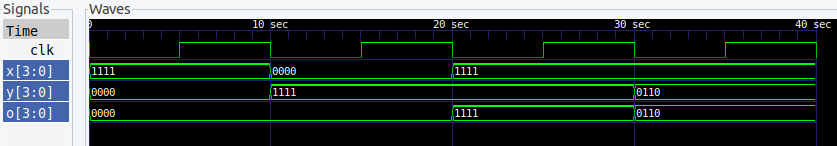
\includegraphics[scale =1.15]{gtk_and_4bit}
	\caption{And Circuit Waveform}
	\label{fig: gtk_and_4bit}
\end{figure}

\begin{figure}[h]
	\centering
	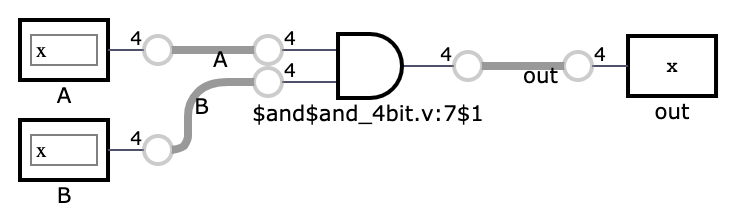
\includegraphics[width=1.0\textwidth]{and_4bit}
	\caption{And Circuit Diagram}
	\label{fig: and_4bit}
\end{figure}
\pagebreak
	\section{Waveform \& Circuit Diagram: Nand Circuit}
	
	The waveform and circuit diagrams for the 4-bit Nand circuit are shown below:

\begin{figure}[h]
	\centering
	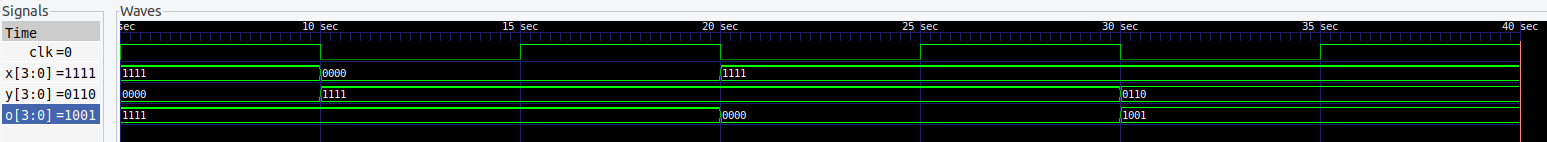
\includegraphics[scale=0.625]{gtk_nand_4bit}
	\caption{Nand Circuit Waveform}
	\label{fig: gtk_nand_4bit}
\end{figure}

\begin{figure}[h]
	\centering
	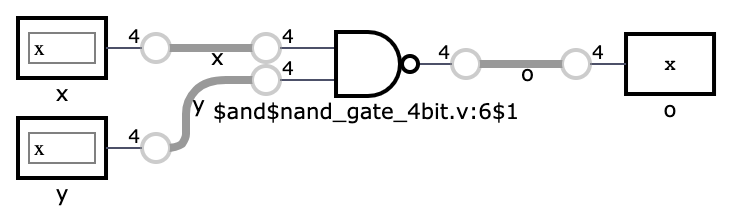
\includegraphics[width=1.0\textwidth]{nand_4bit}
	\caption{Nand Circuit Diagram}
	\label{fig: nand_4bit}
\end{figure}
\pagebreak

	
	\section{Waveform \& Circuit Diagram: Or Circuit}
	
	The waveform and circuit diagrams for the 4-bit Or circuit are shown below:
\begin{figure}[h]
	\centering
	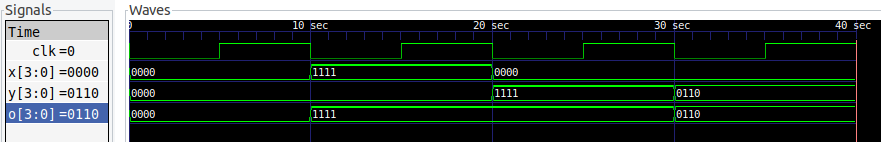
\includegraphics[scale=1.1]{gtk_or_4bit}
	\caption{Or Circuit Waveform}
	\label{fig: gtk_or_4bit}
\end{figure}

\begin{figure}[h]
	\centering
	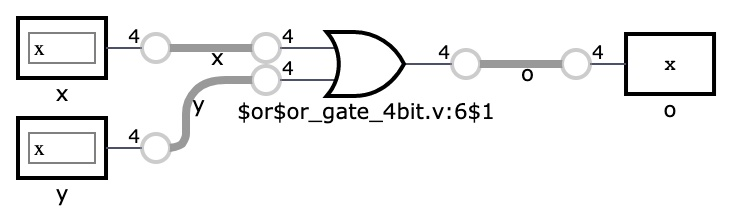
\includegraphics[width=1.0\textwidth]{or_4bit}
	\caption{Or Circuit Diagram}
	\label{fig: or_4bit}
\end{figure}
\pagebreak

	\section{Waveform \& Circuit Diagram: Nor Circuit}
	
	The waveform and circuit diagrams for the 4-bit Nor circuit are shown below:
	
\begin{figure}[h]
	\centering
	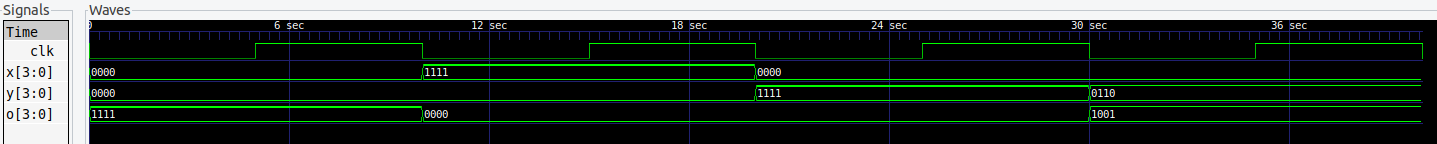
\includegraphics[scale=0.65]{gtk_nor_4bit}
	\caption{Nor Circuit Waveform}
	\label{fig: gtk_nor_4bit}
\end{figure}

\begin{figure}[h]
	\centering
	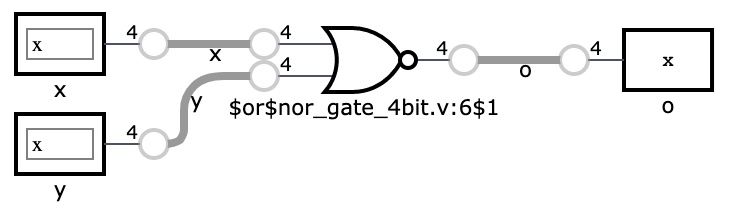
\includegraphics[width=1.0\textwidth]{nor_4bit}
	\caption{Nor Circuit Diagram}
	\label{fig: nor_4bit}
\end{figure}
\pagebreak

	\section{Waveform \& Circuit Diagram: Xor Circuit}
	
	The waveform and circuit diagrams for the 4-bit Xor circuit are shown below:
	
\begin{figure}[h]
	\centering
	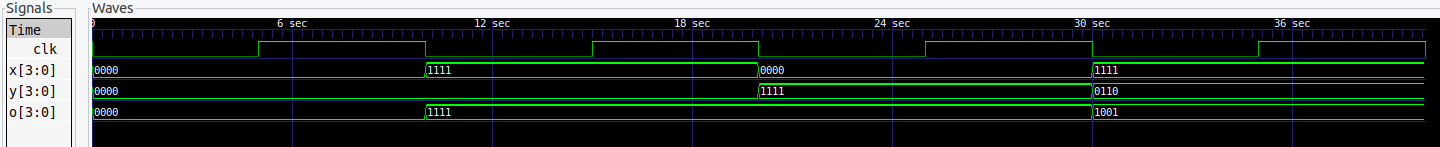
\includegraphics[scale=0.65]{gtk_xor_4bit}
	\caption{Xor Circuit Waveform}
	\label{fig: gtk_xor_4bit}
\end{figure}
	
\begin{figure}[h]
	\centering
	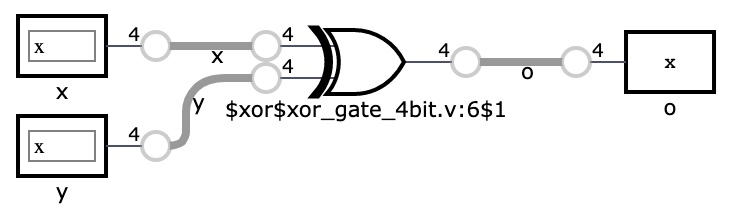
\includegraphics[width=1.0\textwidth]{xor_4bit}
	\caption{Xor Circuit Diagram}
	\label{fig: xor_4bit}
\end{figure}
\pagebreak

	\section{Waveform \& Circuit Diagram: Xnor Circuit}
	
	The waveform and circuit diagrams for the 4-bit Xnor circuit are shown below:
\begin{figure}[h]
	\centering
	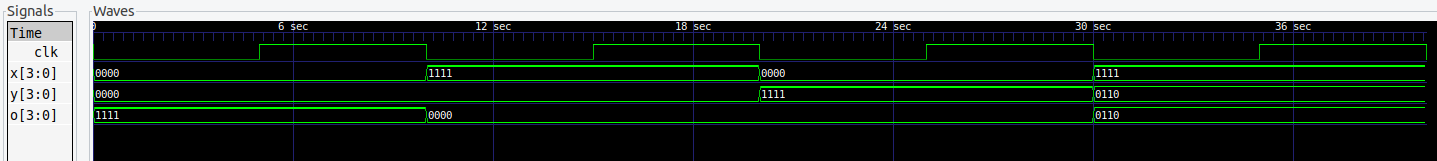
\includegraphics[scale=0.65]{gtk_xnor_4bit}
	\caption{Xnor Circuit Waveform}
	\label{fig: gtk_xnor_4bit}
\end{figure}
	
\begin{figure}[h]
	\centering
	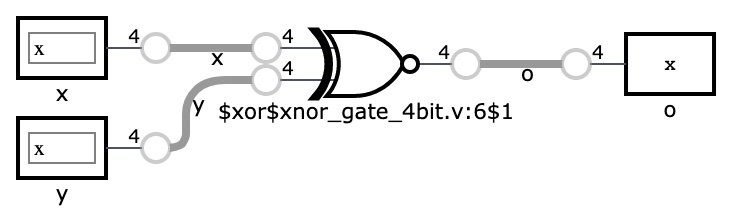
\includegraphics[width=1.0\textwidth]{xnor_4bit}
	\caption{Xnor Circuit Diagram}
	\label{fig: xnor_4bit}
\end{figure}
\pagebreak

	\section{Waveform \& Circuit Diagram: Not Circuit}
	
	The waveform and circuit diagrams for the 4-bit Not circuit are shown below:
	
\begin{figure}[h]
	\centering
	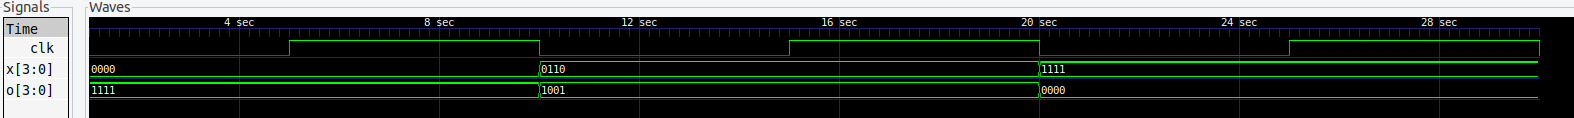
\includegraphics[scale=0.625]{gtk_not_4bit}
	\caption{Not Circuit Waveform}
	\label{fig: gtk_not_4bit}
\end{figure}

\begin{figure}[h]
	\centering
	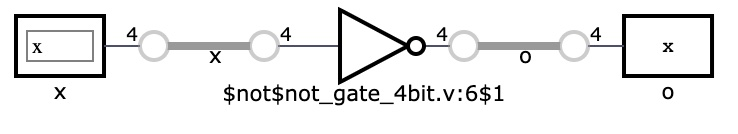
\includegraphics[width=1.0\textwidth]{not_4bit}
	\caption{Not Circuit Diagram}
	\label{fig: not_4bit}
\end{figure}
\pagebreak

	\section{Waveform \& Circuit Diagram: Shifter Circuit}	
	
	The waveform and circuit diagrams for the 4-bit Shifter circuit are shown below:

\begin{figure}[h]
	\centering
	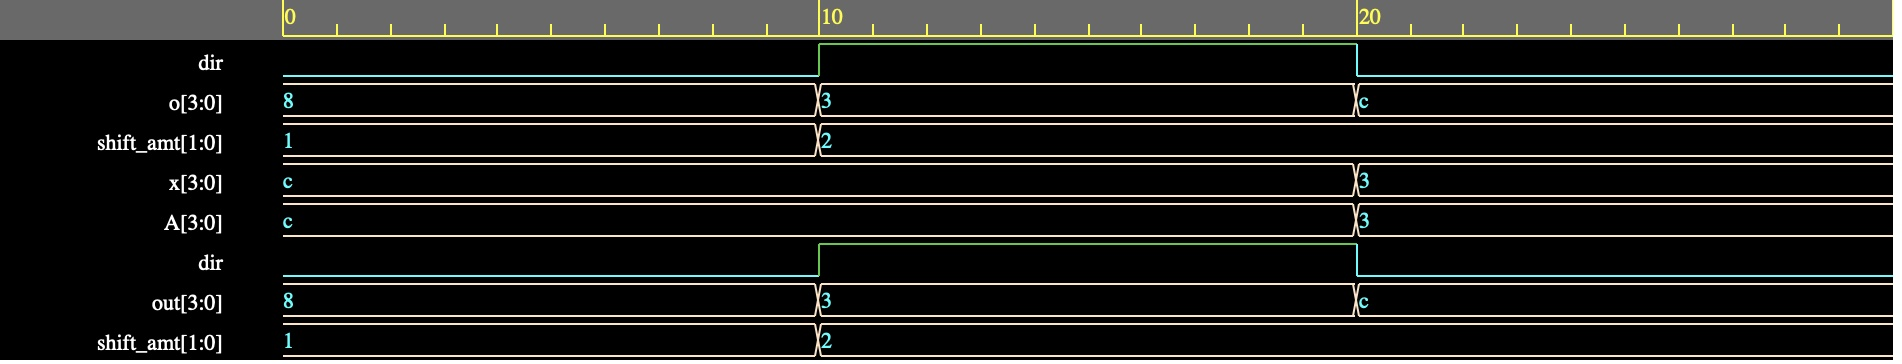
\includegraphics[scale=0.25]{Shifter_waveform}
	\caption{Shifter Circuit Waveform}
	\label{fig: Shifter_waveform}
\end{figure}

\begin{figure}[h]
	\centering
	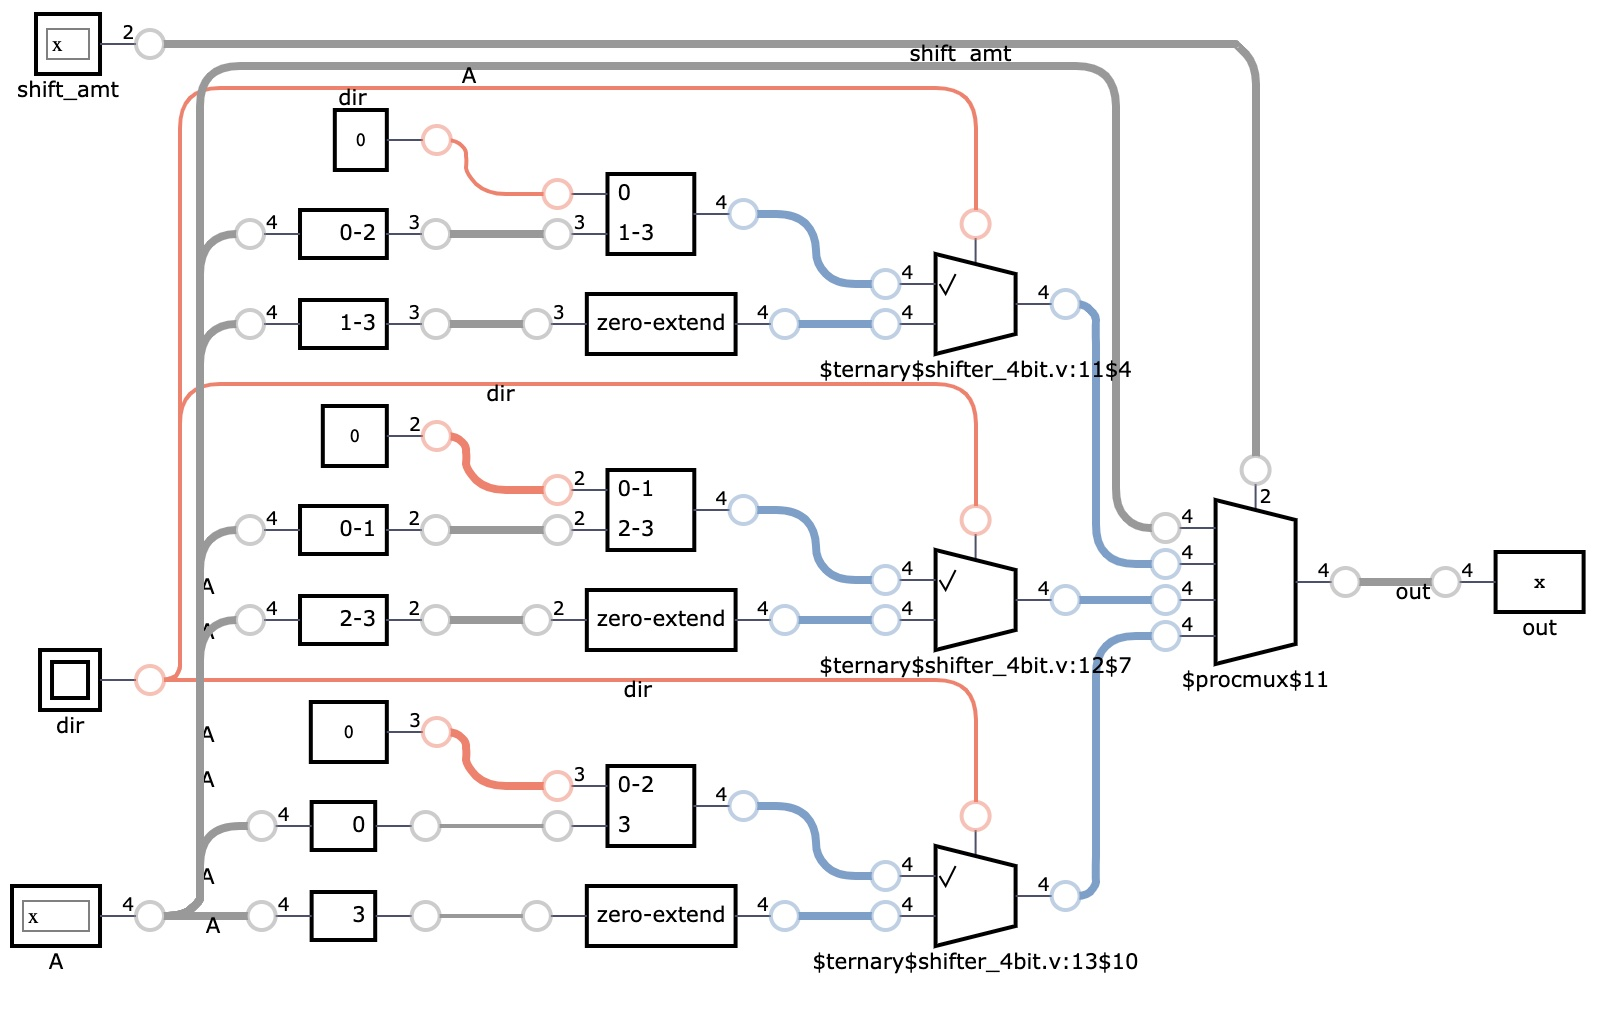
\includegraphics[width=1.0\textwidth]{Shifter_4bit}
	\caption{Shifter Circuit Diagram}
	\label{fig: Shifter_4bit}
\end{figure}
\pagebreak

\section{Waveform \& Circuit Diagram: Addition Circuit}	

The waveform and circuit diagrams for the 4-bit Shifter circuit are shown below:

\begin{figure}[h]
	\centering
	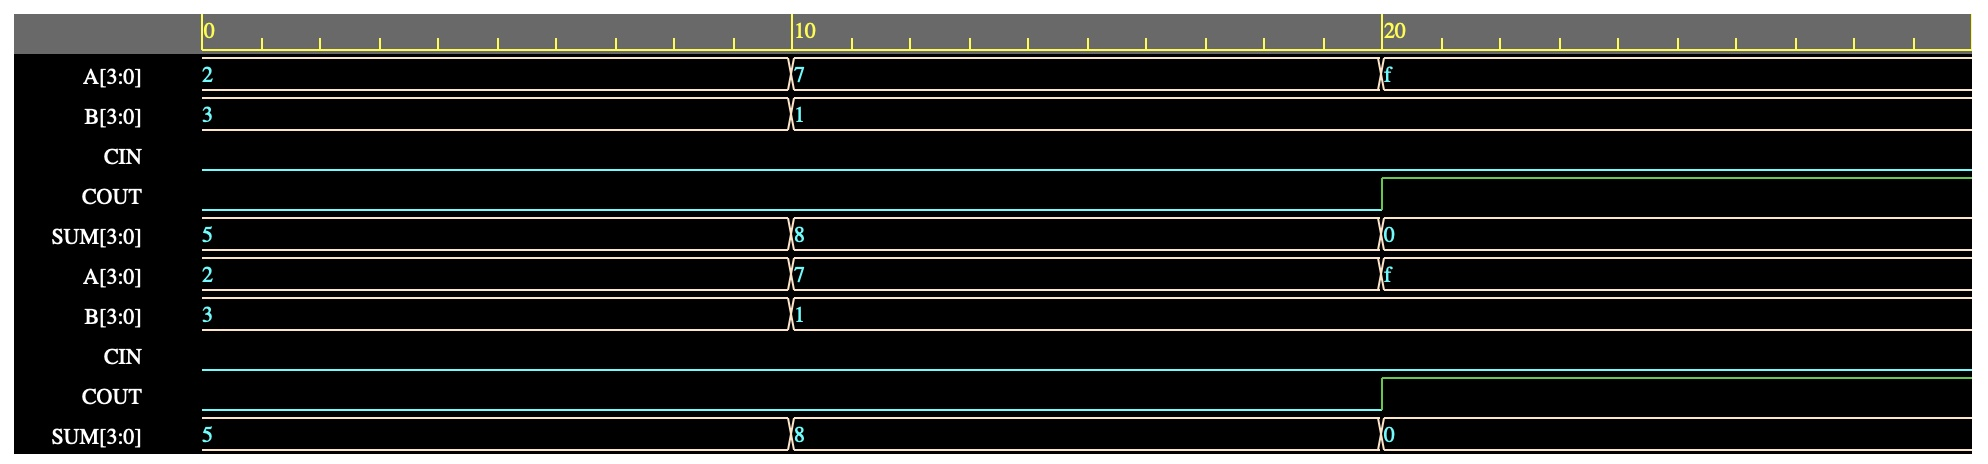
\includegraphics[scale=0.25]{adder_waveform}
	\caption{Adder Circuit Waveform}
	\label{fig: adder_waveform}
\end{figure}

\begin{figure}[h]
	\centering
	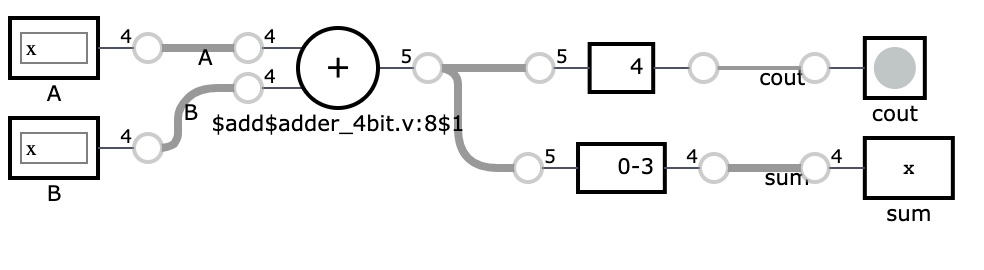
\includegraphics[width=1.0\textwidth]{adder_4bit}
	\caption{Addition Circuit Diagram}
	\label{fig: adder_4bit}
\end{figure}	
\pagebreak

\section{Waveform \& Circuit Diagram: Subtraction Circuit}	

The waveform and circuit diagrams for the 4-bit Shifter circuit are shown below:

\begin{figure}[h]
	\centering
	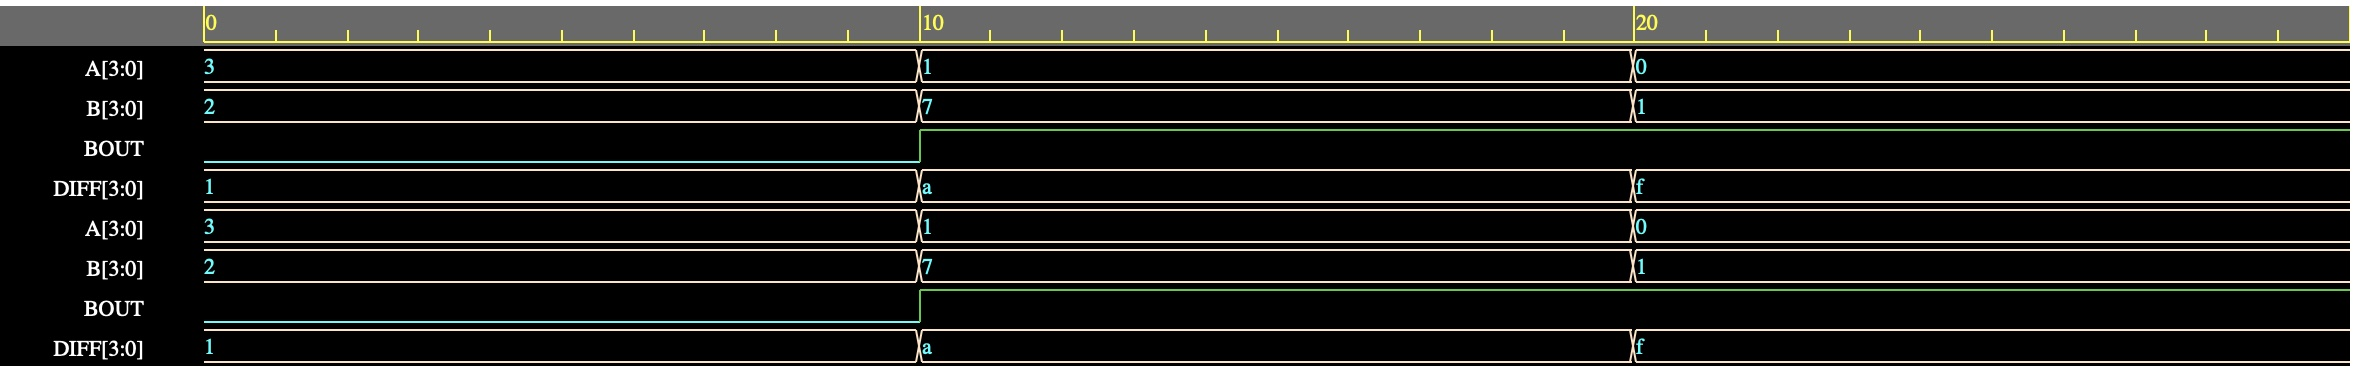
\includegraphics[scale=0.2]{subtractor_waveform}
	\caption{Subtraction Circuit Waveform}
	\label{fig: subtractor_waveform}
\end{figure}

\begin{figure}[h]
	\centering
	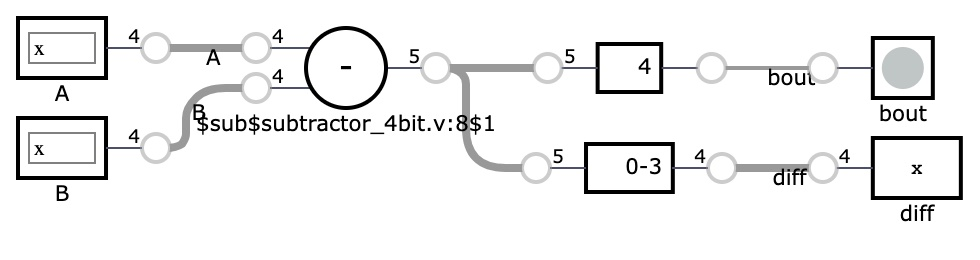
\includegraphics[width=1.0\textwidth]{subtractor_4bit}
	\caption{Subtractor Circuit Diagram}
	\label{fig: subtractor_4bit}
\end{figure}
\pagebreak

\section{Waveform \& Circuit Diagram: Mutliplication Circuit}	

The waveform and circuit diagrams for the 4-bit Shifter circuit are shown below:

\begin{figure}[h]
	\centering
	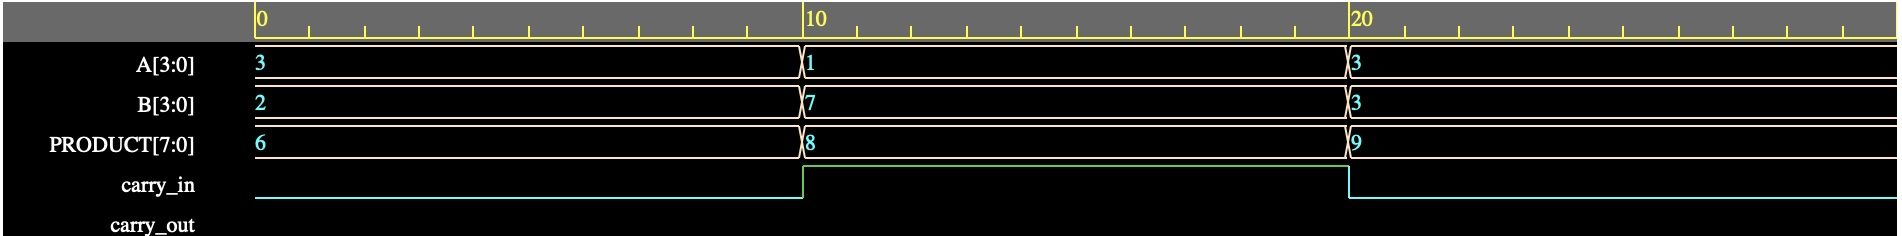
\includegraphics[scale=0.25]{multiplier_waveform}
	\caption{Multiplication Circuit Waveform}
	\label{fig: multiplier_waveform}
\end{figure}

\begin{figure}[h]
	\centering
	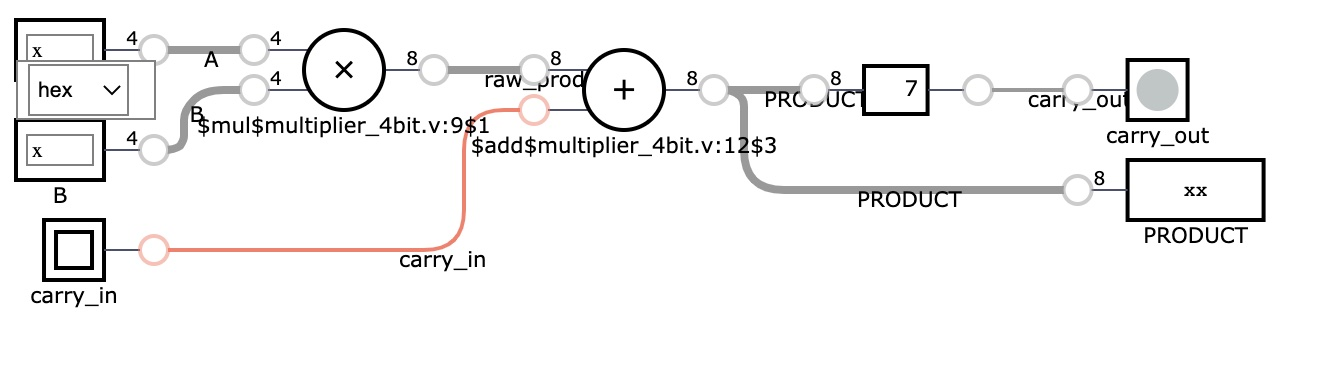
\includegraphics[width=1.0\textwidth]{multiplier_4bit}
	\caption{Multiplication Circuit Diagram}
	\label{fig: multiplier_4bit}
\end{figure}
\pagebreak

\section{Conclusion}

	Given the requirements for this second project status report, I believe our group got the correct results. The code, test, benches, and waveforms for the 4-bit Binary and 4-bit Arithmetic circuits seems to follow the truth tables and outputs for their corresponding logical and arithmetic operations and inputs, so it seems reasonable that they are correct and out project remains successful and on the right track so far. Because we did not have to set up our virtual environments or do much troubleshooting with the tools we are using, such as Verilog or GTK Wave, we did not run into many obstacles or difficulties while working on this project, and we were able to fairly split up the workload between the three of us quickly and fairly. Once the operations were coded and compiled in Verliog, generating the waveforms in GTK Wave and creating the circuit diagrams was fairly straightforward, and all that was left was to gather all the data we created and write the report according to the project requirements.   
	
	
\end{document}
	